\chapter{Bivariate Analysis}
\label{ch:bivariate-analysis}

In previous chapters, we examined one variable at a time. In this chapter we will study the \emph{relationship}\index{relationship} (also: \emph{correlation}\index{correlation} or \emph{association}\index{association}) between variables. We speak of a relationship between two variables when the value of one variable systematically changes depending on the value of the other. In other words, it determines to what extent it becomes easier to predict the value of one variable based on the value of the other variable.

\section{Learning Goals}
\label{sec:bivariate-analysis-learning-goals}

By the end of this chapter you must be able to:

\begin{itemize}
    \item Explain the following concepts:
    \begin{itemize}
        \item dependent variable, independent variable;
        \item a relationship (correlation, association) between two variables, increasing/decreasing relationship, linear relationship;
    \end{itemize}
    \item Identify suitable analysis techniques for the combinations of measurement levels discussed in this chapter;
    \item For a combination of two qualitative variables:
    \begin{itemize}
        \item Create a cross table and apply Cochran's rule;
        \item Calculate the $\chi^2$ statistic;
        \item Apply the $\chi^2$-test (for association and goodness-of-fit);
        \item Calculate and interpret standardized residuals;
        \item Calculate the value of Cramér's V and interpret the result
    \end{itemize}
    \item For a combination of a qualitative independent and a quantitative dependent variable:
    \begin{itemize}
        \item Apply the correct variant of the $t$-test for two samples (paired, independent);
        \item Calculate the effect size (Cohen's $d$) and interpret the result;
    \end{itemize}
    \item For a combination of two quantitative variables:
    \begin{itemize}
        \item determine the equation of the regression line and plot it;
        \item calculate the covariance, the correlation coefficient and the coefficient of determination and describe the value using the correct terms;
    \end{itemize}
    \item Identify and apply appropriate visualization techniques for the combinations of measurement levels discussed in this chapter;
    \item Interpret a given graph consisting of two variables, a.o.~naming the graph type, deducing whether there is a relationship, what type of relationship and the correlation (weak, moderate, strong).
    \item Explain, based on a given situation, that correlation does not imply a causal relationship, and why;
\end{itemize}

\section{Introduction}
\label{sec:bivariate-analysis-introduction}

When describing a relationship between variables, we make a distinction between:

\begin{itemize}
    \item The \emph{dependent variable}\index{variable!dependent}, for which we want to predict the value;
    \item The \emph{independent variable}\index{variable!independent}, for which we know the value and use this value to make a prediction.
\end{itemize}

So if the value of the independent variable changes in a certain way, we expect the value of the dependent variable to change in a predictable way.

\begin{example}
    An example in which relationships can be found between variables is Ant Colony Optimization (ACO), a technique used in various computational problems. The technique is based on how ants search for, and find food, and how they communicate this to the group. Ants spread pheromones when they go out looking for food. The longer the path, the less pheromones the path will contain, the shorter the path, the more likely a large concentration of pheromones can be found. Other ants are attracted by these pheromones and will therefore follow the most traveled paths to get to a particular food source. We can now research whether the time required for finding a path has a relationship with one of the following variables:
    
    \begin{itemize}
        \item The extent to which pheromones are distributed
        \item The degree to which a pheromone disappears
        \item The number of obstacles between the ant nest and the food source
        \item The shape of the obstacles between the nest and source (e.g. do ants find a path faster if the obstacles have no corners)
    \end{itemize}
\end{example}

To investigate whether there is a relationship between two variables, different analysis and visualization techniques can be used, depending on the measurement level. Table~\ref{tab:bivariate_analysis} provides an overview of suitable analysis techniques discussed in this syllabus, and Table~\ref{tab:bivariate_visualization} of suitable graph types.

However, note that there are many other analysis techniques that are not discussed in this syllabus! This syllabus only provides a sneak preview\ldots If later during your career, you need to use statistical techniques (the authors of this syllabus strongly believe that this can happen effectively), we recommend spending some time researching wether there exist better techniques for your specific research question.

\begin{table}
    \begin{tabular}{llll}
        \toprule
        \textbf{Independent}    & \textbf{Dependent}    & \textbf{Test}                 & \textbf{Metric}         \\
        \midrule
        Qualitative             & Qualitative           & $\chi^2$-test                 & Cramér's $V$            \\
        Qualitative             & Quantitative          & two-sample $t$-test           & Cohen's $d$             \\
        Quantitative            & Quantitative          & ---                           & Regression, correlation \\
        \bottomrule
    \end{tabular}
    \caption{Overview of techniques for analysing the relationship between two variables. The table provides the suitable statistical tests, and the metrics that can be used to express the relationship.}
    \label{tab:bivariate_analysis}
\end{table}

\begin{table}
    \begin{tabular}{lll}
        \toprule
        \textbf{Independent}    & \textbf{Dependent}    & \textbf{Graph Type}                                  \\
        \midrule
        Qualitative             & Qualitative           & Mosaic plot, horizontal stacked bar chart, clustered bar chart \\
        Qualitative             & Quantitative          & Boxplot, bar chart with error bars                  \\
        Quantitative            & Quantitative          & Scatter plot, regression line                    \\
        \bottomrule
    \end{tabular}
    \caption{Overview of techniques for visualizing the relationship between two variables.}
    \label{tab:bivariate_visualization}
\end{table}

\section{Qualitative--Qualitative}
\label{sec:qualitative-qualitative}

In this section we investigate methods for researching the relationship between two qualitative variables. All methods are based on a summarizing table of frequencies of the variables, the cross table (cfr. Section~\ref{ssec:cross-tables}). Based on this, a statistic is calculated that expresses how great the differences are between the two variables, the so-called ``Chi-squared'', notation $\chi^2$\footnote{Chi, $\chi$ is a letter from the Greek alphabet.} (cfr. Section~\ref{ssec:chi-square}). The $\chi^2$-test (cfr. Section~\ref{ssec:test-of-independence} and Section~\ref{ssec:goodness-of-fit-test}) can be used to determine wether the value of $\chi^2$ indicates that there is a relationship between the two variables. There is also another technique, Cramér's $V$ (cfr. Section~\ref{ssec:cramers-v}), which reduces the value of $\chi^2$ to a number between 0 and 1, and can be used to derive the strength of the relationship.

\subsection{Cross Tables}
\label{ssec:cross-tables}

\begin{definition}[Cross Table]
    A cross table\index{cross table}\index{table!cross} (also called contingency table\index{table!contingency}, cross tabulation or crosstab) summarizes the frequencies of two variables.
    
    Each cell of the last column contains the sum of the corresponding row, and each cell of the last row contains the sum of the corresponding column. These values are called the \emph{marginal totals}\index{total!marginal}\index{marginal total}.
\end{definition}

\begin{table} \centering
    \begin{tabular}{@{}rrrr}
        \toprule
              & Women & Men &  Total \\
        \midrule
         Good &     9 &   8 &     17 \\
   Sufficient &     8 &  10 &     18 \\
 Insufficient &     5 &   5 &     10 \\
          Bad &     0 &   4 &      4 \\
        Total &    22 &  27 &     49 \\
        \bottomrule
    \end{tabular}
    \caption{A cross table for the appreciation by men and women of a particular range of products.}
    \label{tab:crosstable0}
\end{table}

How can we determine, based on a cross table, whether there is a relationship between two variables? For example, take a look at the cross table of Table~\ref{tab:crosstable0}. This table summarizes the results of a survey in which 49 persons (22 woman and 27 men) were asked to give a rating (good, sufficient, bad) for a particular range of products. If there is a relationship between the two variables, namely the gender (independent) and the rating (dependent), we should be able to see that women and men gave fundamentally different ratings. On the other hand, if the proportions of the different ratings are (approximately) the same for both women and men, there is \emph{no} relationship.

An ordinary cross table cannot be directly used for drawing conclusions, as analyzing a possible coherence between variables is not straightforward based on absolute frequencies. After all, there are more men than women in the survey! Instead, we have to calculate the percentages, i.e.~within each column we need to calculate how often each rating occurs \emph{in proportion}. The sum of all percentages in a column needs to be equal to 100\%. A quick review of the rules regarding calculating percentages:

\begin{itemize}
  \item To determine what percent $x$ is of $y$, divide $x$ by $y$ and multiply by 100: $p = \frac{x}{y} \times 100$. For example: what percentage is 15 of 20? $\frac{15}{20} \times 100 = 75$, so 75\%.
  \item To calculate $x\%$ of $y$: $\frac{x \times y}{100}$. For example: calculate 60\% of 30? $\frac{60 \times 30}{100} = 18$.
\end{itemize}

Table~\ref{tab:crosstable1} provides an overview of the percentages per gender for each appreciation that occured in the sample. For example, we see that 41\% of women gave a good rating (because 9 is approximately 41\% of 22), compared to 30\% of men.

\begin{table} \centering
  \begin{tabular}{@{}rrrrrrr@{}}
  	\toprule
                & Women & Men &  Total & Women \% & Men\% & Total  \\
  	\midrule
  	       Good &     9 &   8 &     17 &     41\% &  30\% &   35\% \\
     Sufficient &     8 &  10 &     18 &     36\% &  37\% &   37\% \\
   Insufficient &     5 &   5 &     10 &     23\% &  18\% &   20\% \\
            Bad &     0 &   4 &      4 &      0\% &  15\% &    8\% \\
  	      Total &    22 &  27 &     49 &    100\% & 100\% &  100\% \\
  	\bottomrule
  \end{tabular}
  \caption{The cross table, including percentages of the different values.}
  \label{tab:crosstable1}
\end{table}

We can now ask ourselves whether the choice of rating depends on the gender of the repondent. There are differences between the two columns, se you could suspect that this is indeed the case. Smaller differences indicate a weak relationship, whereas greater differences indicate a stronger coherence.

\subsection{\texorpdfstring{$\chi^{2}$}{chi-square}}
\label{ssec:chi-square}

The previous section indicates the need for a measure to express the difference between the ratios in both columns. One way to express this is the so-called \emph{chi-square} statistic (notation: $\chi^{2}$). The value of $\chi^2$ equals 0 when there is no difference between the proportions in the columns of a cross table, and therefore when there is absolutely no coherence between the variables. If there is a difference, $\chi^2$ will be a positive number. The larger the value, the greater the mutual differences between both columns, and the stronger the relationship.

The procedure for calculating the value of $\chi^2$ based on a cross table is as follows:

\begin{enumerate}
  \item First, create a cross table containing the marginal totals (cfr. Table.\ref{tab:crosstable0}).
  \item Next, calculate the so-called \emph{expected frequency} of each cell (notation: $e$). This is the absolute frequency you would \emph{expect} if you assume there is no relationship at all between the variables. You can calculate the expected frequency as follows:
  
  \begin{equation}
      e = \frac{row total \times column total}{n}
  \end{equation}

  with:

  \begin{itemize}
      \item $row total$ the sum of all values of the cell's row
      \item $column total$ the sum of all values of the cell's column
      \item $n$ the number of observations
  \end{itemize}

  For cell$_{1,2}$ (the expected number of man that answered ``good'') this corresponds to $\frac{17 \times 27}{49} \approx 9.37\%$.

  \item Next you calculate the difference between the \emph{observed} (notation: $o$) and the \emph{expected} frequency ($e$). (cfr. Table~\ref{tab:crosstable2}).

  \begin{table} \centering
    \begin{tabular}{@{}rrrrrrr@{}}
      \toprule
                &                       Women &                          Men &  Total & Women \% &   Men\% &   Total \\
      \midrule
           Good &  $9 -\textcolor{red}{7.63}$ &  $8 - \textcolor{red}{9.36}$ &   $17$ &   $41$\% &  $30$\% &  $35$\% \\
     Sufficient & $8 - \textcolor{red}{8.08}$ & $10 - \textcolor{red}{9.91}$ &   $18$ &   $36$\% &  $37$\% &  $37$\% \\
   Insufficient & $5 - \textcolor{red}{4.48}$ &  $5 - \textcolor{red}{5.51}$ &   $10$ &   $23$\% &  $18$\% &  $20$\% \\
            Bad & $0 - \textcolor{red}{1.79}$ &  $4 - \textcolor{red}{2.20}$ &    $4$ &    $0$\% &  $15$\% &   $8$\% \\
          Total &                        $22$ &                         $27$ &   $49$ &  $100$\% & $100$\% & $100$\% \\
    \bottomrule
    \end{tabular}
    \caption{The cross table, with the expected frequency $e$ (indicated in red) subtracted from the observed frequency $o$ for each cell.}
    \label{tab:crosstable2}
  \end{table}

  \item The final step involves calculating a measure for the dispersion of each cell. Similar to calculating the variance of a sample (cfr. Section~\ref{ssec:variance-and-standard-deviation}), we calculate the squared difference so that the result is always positive and larger deviations will have a greater influence in the result.

  We will also divide the dispersion by the expected frequency to make them both relatively equally important. For example: a standard deviation of 5 for an expected frequency of 20 is bigger than for an expected frequency of 200. The resulting equation for each cell of the cross table is (cfr. Table~\ref{tab:crosstable3}):

  \begin{equation}
    \frac{(o - e)^{2}}{e}
  \end{equation}

  \begin{table} \centering
    \begin{tabular}{@{}rrrrrrr@{}}
      \toprule
                &                    Women &                      Men &  Total & Women \% &   Men\% &   Total \\
    	\midrule
           Good & $\textcolor{blue}{0.24}$ & $\textcolor{blue}{0.20}$ &   $17$ &   $41$\% &  $30$\% &  $35$\% \\
     Sufficient & $\textcolor{blue}{0.00}$ & $\textcolor{blue}{0.00}$ &   $18$ &   $36$\% &  $37$\% &  $37$\% \\
   Insufficient & $\textcolor{blue}{0.06}$ & $\textcolor{blue}{0.05}$ &   $10$ &   $23$\% &  $18$\% &  $20$\% \\
            Bad & $\textcolor{blue}{1.80}$ & $\textcolor{blue}{1.46}$ &    $4$ &    $0$\% &  $15$\% &   $8$\% \\
          Total &                     $22$ &                     $27$ &   $49$ &  $100$\% & $100$\% & $100$\% \\
    	\bottomrule
    \end{tabular}
    \caption{The cross table, with the squared difference divided by the expected frequency, $\frac{(o - e)^2}{e}$ (in blue). Note that these values are rounded to two decimal places, so we lose some of the precision.}
    \label{tab:crosstable3}
  \end{table}

  \item Finally, we take the sum of all values to determine the value of $\chi^{2}$:
  \item 
  \begin{equation}
    \chi^{2} = \sum \frac{(o - e)^{2}}{e}
    \end{equation}
    
    In our example: $\chi^2 \approx 3.8105$.
\end{enumerate}

However, this value $\chi^2 \approx 3,8105$ itself \emph{still} does not say much. Under what conditions can we say whether there is a relationship between the two variables? And how strong is this relationship? This will also depend on the size of the table and the total number of observations. In a cross table consisting of more rows/columns, the value of $\chi^2$ will have to be larger to conclude that there is a relationship.

\subsection[Chi-squared Distribution]{$\chi^{2}$-distribution}
\label{ssec:chi-squared-distribution}

In Section~\ref{ssec:test-of-independence} we will introduce the $\chi^2$-test. This test uses the so-called $\chi^2$-distribution for determining the probability value or critical value. Although $\chi^2$-distribution does not occur in nature, and therefore few phenomenoms can be modeled using this distribution, it is \emph{very} useful in this \emph{context}.

Assume that  $X_{1}, X_{2}, \dots X_{v}$ are independent variables with a standard normal distribution ($\sim N(0,1)$). The $\chi^{2}$ (chi-square) variable is then defined as follows:

\[ \chi^{2}_{v} = X_{1}^{2} + X_{2}^{2} + \dots + X_{v}^{2} \]

The value of $v$ is the number of degrees of freedom of the variable. $\chi^{2}$ is a continuous random variable, and has a positive value because it is calculated by taking the sum of the squared differences. The distribution function is as follows:

\[ f_{n}(x) = \frac{1}{2^{\frac{n}{2}}\Gamma(\frac{n}{2})} x^{\frac{n}{2} -1} e^{\frac{x}{2}} \]

The expected value (= mean) is $v$ with a variance $2v$. The mode of $v \geq 2$ is $v-2$.

To determine the necessary values within the $\chi^{2}$-distribution (e.g. right-tailed probability, critical value), we can either use a table \footnote{For example \url{https://people.richland.edu/james/lecture/m170/tbl-chi.html}}, or statistical software such as R.

\begin{figure}
  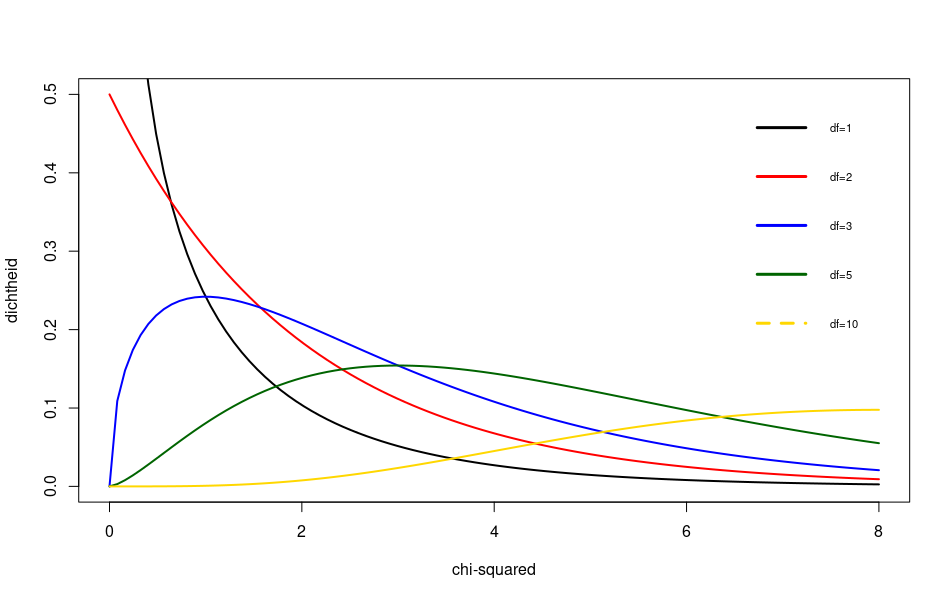
\includegraphics[width=\textwidth]{chi-squared-distribution}
  \caption{Density function of the$\chi^2$-distribution for different degrees of freedom $df$.}
  \label{fig:chi-squared-distribution}
\end{figure}

\subsection{Test of Independence}
\label{ssec:test-of-independence}

A test of independence\index{test of independence} is used to determine if there is a relationship between two qualitative variables by using the $\chi^2$ statistic. This test is also called the $\chi^2$-test\index{$\chi^2$-test}\index{test!$\chi^2$-} of association, or the $\chi^2$ cross table test, and was developed by the English mathematician and statistician Karl Pearson\index{Pearson!Karl}.

\subsubsection{Testing Procedure}

The testing procedure is as follows:

\begin{enumerate}
  \item \textbf{Formulate both hypotheses}
  As a null hypothesis, we state that there is no relationship between the independent and the dependent variable (so we expect a small value for $\chi^2$).
  As alternative hypothesis, we state that there \emph{is} a relationship (and therefore we expect $\chi^2$ to be large).
  \begin{itemize}
    \item $H_{0}$: There is no relationship between the variables (or: the variables are independent)
    \item $H_{1}$: There is a relationship between the variables
  \end{itemize}

  \item \textbf{Determine significance level $\alpha$}
  
  \item \textbf{Calculate the value of the test statistic in the sample}
  \[ \chi^{2} = \sum_{i} \frac{(o_{i} - e_{i})^{2}}{e_{i}} \]

  \item The value of $\chi^2$ follows the $\chi^2$-distribution (cfr. Section~\ref{ssec:chi-squared-distribution}). This stochastic distribution has an additional parameter, the number of degrees of freedom $df$. For a cross table test, $df = (r - 1) \times (k - 1)$ with $r$ the number of rows and $k$ the number of columns.

  Using this distribution, we can draw a conclusion in two equivalent ways:
  \begin{enumerate}
    \item \textbf{Calculate and plot the critical area}. The critical value $g$ is the value for which $P(\chi^2 > g) = \alpha$. This test is always right-tailed. If $\chi^2 < g$, we are inside the \emph{region of acceptance}, and we cannot reject the null hypothesis. If $\chi^2 > g$, we are inside the \emph{region of rejectance} or \emph{critical region} and we will reject the null hypothesis.
    \item \textbf{Calculate the probability value $p$}. This is the right-tail probability for the $\chi^2$ statistic in the sample, depending on the number of degrees of freedom. The interpration of the $p$-value is ``If we assume that there is \emph{no} relationship between the two variables, what is the probability of obtaining a value for $\chi^2$ in a sample that is as least as large as the obtained one?'' If $p > \alpha$ (and therefore there is a relatively great probability to obtain this $\chi^2$-value), we accept the null hypothesis, if $p < \alpha$, we reject it.
  \end{enumerate}

  \item Finally, we formulate the conclusion and answer the research question.
\end{enumerate}  

Applied to the previous example:

\begin{enumerate}
  \item \textbf{Formulate both hypotheses:}
  \begin{itemize}
    \item $H_0$ There is no relationship between gender and rating
    \item $H_1$ There is a relationship between gender and rating
  \end{itemize}
  \item \textbf{Determine significance level:} $\alpha = 0.05$
  
  \item \textbf{Calculate the value of the test statistic in the sample}
  
  $\chi^2 \approx 3.8105$ (cfr. Section~\ref{ssec:chi-square})
  
  \item Determine the number of degrees of freedom $df = (r - 1) \times (k - 1) = (4 - 1) \times (2 - 1) = 3$.
  
  \begin{enumerate}
    \item \textbf{Calculate the critical value:} $g \approx 7.815$. In this case $\chi^2 < g$, so we are inside the region of acceptance. Therefore we cannot reject $H_0$.
    \item \textbf{Calculate the probability value:} $p \approx 0.2827$. There is a probability of around 28\% to obtain this $\chi^2$-value from a sample. That is quite large, certainly larger than $\alpha$. As a result we cannot reject $H_0$.
  \end{enumerate}

  \item We can therefore assume that, based on this sample, there is no reason to assume that there is a relationship between gender and rating. In other words, there are no significant differences between the ratings given by women and men.
\end{enumerate}


We investigate another example of the test of independence based on a study by \textcite{Doll1954} regarding the relationship between smoking and cancer. In 1951, Doll and Hill wrote to all British general practitioners (GPs) requesting information about their age and smoking behavior. Next, they tracked death reports and cause of death over years and repeated this periodically. The first results, after around four years, are summarized in Table~\ref{tab:dollhill}. It can easily be concluded from this table that there is no relationship between smoking and lung cancer. In (over) four years, only $(84 / 24354) * 100 = 0.35\%$ of British GPs died of lung cancer, and this with only $(83 / 21261) * 100 = 0.39\%$ of smokers among them. This result is small, but it is much larger than the result for the non-smokers $(1 / 3093) * 100 = 0,032\%$.

\begin{table}
  \begin{center}
    \begin{tabular}{@{}lllll@{}}
    	\toprule
    	                & \textbf{Lung Cancer} & \textbf{No} & \textbf{Yes} & \textbf{Total} \\
    	\midrule
    	\textbf{Smoker} & \textbf{Yes}         & 21178       & 83           & 21261           \\
    	                & \textbf{No}          & 3092        & 1            & 3093            \\
    	                & \textbf{Total}       & 24270       & 84           & 24354           \\
    	\bottomrule
    \end{tabular}
  \end{center}
  \caption{Results of the research of~\textcite{Doll1954}}
  \label{tab:dollhill}
\end{table}

The table illustrates thate there is a significant difference between the observed number of smokers that died of lung cancer and the expected frequencies in this cell. The same applies to the small number of GPs who do not smoke, but who have died of lung cancer. This observation makes us suspicious whether the earlier tentative conclusion is correct. We can deal with this uncertainty by calculating the test statistic $\chi^{2}$. We do this in the familiar way:

\begin{enumerate}
  \item \textbf{Formulate both hypotheses:}
  \begin{itemize}
    \item $H_{0}$: There is no relationship between smoking and dying from lung cancer
    \item $H_{1}$: There is a relationship between smoking and dying from lung cancer
  \end{itemize}
  \item \textbf{Determine $\alpha$ and $n$:} $\alpha = 0.05$ and $n = 24354$.
  \item \textbf{Calculate the value of the test statistic in the sample}:
  \[ \chi^{2} = \sum_{i=1}^{k \times r} \frac{(o_{i} - e_{i})^{2}}{e_{i}} \approx 10.071 \]
  \item \textbf{Calculate and plot the critical area}: The number of degrees of freedom is $df = (r-1)(k-1) = 1$, so for the selected significance level the critical value is 3.8415. Our test statistic is inside the critical region so we reject $H_{0}$.
\end{enumerate}

We must therefore reject $H_{0}$, which states that there is no relationship between the two variables, in favor of $H_{1}$, which states that there is a relationship between the two variables: smokers are more likely to die of lung cancer compared to non-smokers.

But, is this evidence that smoking \emph{causes} lung cancer, as is often assumed? No, it is absolutely not. A few alternative explanations: not all smokers get lung cancer, smokers are older than non-smokers, smokers often live in large cities with more polluted air than non-smokers who often live in the countryside, and there could also be a special genetic disposition which affects both tobacco addiction as well as the chance of developing lung cancer. For a causal interpretation of the data (note, after all, this is not an experiment), we should at least have a theory that makes the relationship between smoking and lung cancer explicit.

\begin{remark}[!!]
  \textbf{Correlation is not causation.} Or in other words, a relationship between two variables does no imply a \emph{causal} relationship. This is a very common mistake made by journalists when writing an article about scientific research results. So be alert when reading such articles!
\end{remark}

\subsubsection{Cochran's Rule}

When calculating the value of $\chi^2$, it is important to have enough observations for each cell in the cross table. When the sample size is too small, the results of the calculation will become unreliable.

The statistician \textcite{Cochran1954}\index{Cochran!William G.} has formulated a number of recommendations about this, which we will refer to in this syllabus as the Rule of Cochran\index{Cochran!rule of}.

More specifically, in order to apply the $\chi^2$-test, the following conditions must be met:

\begin{enumerate}
  \item For all categories, the expected frequency $e$ must be greater than 1.
  \item In a maximum of 20 \% of the categories, the expected frequency $e$ may be less than 5.
\end{enumerate}

\subsection{Goodness Of Fit Test}
\label{ssec:goodness-of-fit-test}

The $\chi^2$-test can also be used when you want to verify whether a given discrete distribution (e.g. the frequencies of a single qualitative variable) corresponds to a known distribution. This variant is called the \emph{goodness of fit test}\index{goodness of fit test}\index{test!goodness of fit}. This test is often used to determine whether the distribution of a given qualitative variable in a sample is representative for the population, assuming that you know the frequencies in the population as a whole.

For example, assume that in the research regarding our superheroes a sample is taken consisting of $n = 400$ observations. The researchers want to determine whether the types of superheroes in the sample match those in the population, or in other words if the sample is representative. Table~\ref{tab:frequencies-types-superheroes} provides an overview of the observed frequencies in the sample and the expected frequencies in the full population.

\begin{table}
  \centering
  \begin{tabular}{@{}lcc@{}}
  	\toprule
  	\textbf{Type}   & \textbf{frq sample ($o$)} & \textbf{frq population ($\pi$)} \\
  	\midrule
  	Mutant          &              127              &              35\%              \\
  	Human           &              75               &              17\%              \\
  	Alien           &              98               &              23\%              \\
  	God             &              27               &              8\%               \\
  	Demon           &              73               &              17\%              \\
  	\midrule
  	\textbf{Total } &              400              &             100\%
  \end{tabular}
  \caption{Absolute frequencies of the observed superhero types in the sample ($o$) and expected relative frequencies ($\pi$) in the full population.}
  \label{tab:frequencies-types-superheroes}
\end{table}

We want to compare the frequencies in the sample with the numbers you would expect if the sample was exactly representative for the superhero types. If these differences are relatively large, the distribution in the sample does \emph{not} match the distribution in the population and we will have to conclude that the sample is not representative. To decide whether these differences are relatively large, we perform a $\chi^{2}$-test.

If the sample is exactly representative, we would expect 35\% of the superheroes in the sample to be a mutant. The expected number or expected frequency for this category is therefore equal to $0.35 \times 400 = 140$. And therefore:

\[ e = n \times \pi \]

with $e$ the expected absolute frequency in the sample, $n$ the sample size and $\pi$ the expected relative frequency for the full population. If the differences between the observed and expected frequencies $(o - e)$ are relatively small, they can be attributed to random sampling errors. We can again use $\chi^2$ to summarize and interpret these differences:

\[ \chi^{2} = \sum_i \frac{(o_{i} - e_{i})^{2}}{e_{i}} \]

Note that:

\begin{itemize}
  \item if the differences are small $\Rightarrow$ distribution is representative
  \item if the differences are large $\Rightarrow$ distribution is not representative
\end{itemize}

We now determine a critical value $g$ which has a $\chi^{2}$ distribution. For this, the number of degrees of freedom plays a role. For this test, the following applies:

\[ df = k - 1 \]

with $k$ the number of categories. In our example, we have that $df = 5-1 = 4$. To determine the critical value, we can use a table of the $\chi^2$-distribution. For a given significance level $\alpha$ and degrees of freedom $df$, the table provides the critical value.

In our example, $\chi^{2} = 3.47$ with critical value $g = 9.49$. Because the resulting test statistic $\chi^2 = 3.47 < g = 9.49$, we can conclude that the sample is representative.

\subsubsection{Testing Procedure}

We follow the steps of a statistical testing procedure:

\begin{enumerate}
  \item \textbf{Formulate both hypotheses}
  As a null hypothesis, we formulate that the sample is representative, or more specifically that the distribution in the sample is equal to the distribution of the population. As an alternative hypothesis, we formulate that the distributions are different.
  \begin{itemize}
    \item $H_{0}$: sample is representative for the population
    \item $H_{1}$: sample is not representative for the population
  \end{itemize}
  \item \textbf{Determine $\alpha$ and $n$}
  \item \textbf{Value of the test statistic in the sample}:
  \[ \chi^{2} = \sum_{i=1}^{n} \frac{(o_{i} - e_{i})^{2}}{e_{i}} \]
  \item Determine the number of degrees of freedom $df = k - 1$ with $k$ the number of categories
  \begin{enumerate}
    \item \textbf{Calculate and plot the critical area}: The test is always right-tailed. If the test statistic is smaller than the critical value $\chi^2 < g$, do not reject $H_{0}$. If $\chi^2 > g$, reject $H_{0}$ and accept $H_{1}$.
    \item \textbf{Calculate the probability value $p$}. If $p > \alpha$, we accept the null hypothesis, if $p < \alpha$, we reject it.
  \end{enumerate}
  \item Finally, formulate an answer for the research question.
\end{enumerate}

\subsubsection{Standardized Residuals}

We investigate another example. Consider all families with exactly 5 children in a given community. When we look at the number of boys/girls in such a family, there are 6 possible combinations:

\begin{enumerate}
  \item 5 boys
  \item 4 boys, 1 girl
  \item 3 boys, 2 girls
  \item 2 boys, 3 girls
  \item 1 boy, 4 girls
  \item 5 girls
\end{enumerate}

Suppose a study was conducted in which 1022 families with 5 children participated. Table~\ref{tab:5-children} provides the frequencies of the number of boys in each family. Are the observed numbers in the 6 classes representative for a population in which the probability of having a boy is equal to the probability of having a girl, or more concrete 0.5?

\begin{table}
  \centering
  \begin{tabular}{@{}cccccccc@{}}
    \toprule
    i       & 0  & 1   & 2   & 3   & 4   & 5  &  \\
    \midrule
    $o_{i}$ & 58 & 149 & 305 & 303 & 162 & 45 &  \\
    \bottomrule
  \end{tabular}
  \caption{Frequencies $o_i$ of the number of boys $i$ in families with 5 children based on a study from $n = 1022$ families.}
  \label{tab:5-children}
\end{table}

If the assumption is true, the probability $\pi_{i}$ to have $i$ boys is determined by a binomial distribution with parameters $n=5$ and $p=0.5$.

You can easily verify this using an example. The probability of having 2 boys out of 5 children is equal to:

\[ (0.5)^{2} \times (1-0.5)^{5-2} \times \binom{5}{2} \]

Or in general:

\[ \pi_{i} = \binom{5}{i}\times 0.5^{i} \times 0.5^{5-i} = \frac{5!}{i!(5-i)!}\times 0.5^{5} \]

Based on this $\pi_{i}$ we can determine the expected frequency $e$ and follow the steps described before. Table~\ref{tab:5-children-calculations} provides an overview of the necessary calculations.

\begin{table}
  \centering
  \begin{tabular}{@{}lrrrrrrr@{}}
  	\toprule
  	$i$                   &     0 &      1 &      2 &      3 &      4 &     5 &  Tot. \\
  	\midrule
  	$o_i$                 &    58 &    149 &    305 &    303 &    162 &    45 &  1022 \\
  	$\pi_i$               &  0.03 &   0.15 &   0.31 &   0.31 &   0.15 & 0.031 &     1 \\
  	$e_i$                 & 31.68 & 159.43 & 318.86 & 318.86 & 159.43 & 31.68 &       \\
  	$\frac{(o-e)^{2}}{e}$ & 21.86 &   0.68 &   0.60 &   0.78 &   0.04 &  5.59 & 29.57 \\
  	$r_i$                 &  4.74 &  -0.89 &  -0.93 & -1.071 &   0.22 &  2.40 &       \\
  	\bottomrule
  \end{tabular}
  \caption{Calculations for the case of families with 5 children. $i$ is the number of boys in the family, $o_i$ the observed number of families in the sample with $i$ boys. $\pi_i$ is the expected probability that a family of 5 children has $i$ boys and $e_i$ the expected frequency. Below, the calculation of $\chi^2$ is shown and finally the standardized residuals $r_i$.}
  \label{tab:5-children-calculations}
\end{table}

\begin{enumerate}
  \item \textbf{Formulate both hypotheses}
  
  \begin{itemize}
    \item $H_{0}$: the sample is representative for the population
    \item $H_{1}$: the sample is not representative for the population
  \end{itemize}
  \item \textbf{Determine $\alpha$ and $n$} : $\alpha = 0.01$ and $n = 1022$.
  \item \textbf{Value of the test statistic in the sample}:
  \[ \chi^{2} = \sum_{i=1}^{n} \frac{(o_{i} - e_{i})^{2}}{e_{i}} = 29.5766 \]
  \item \textbf{Calculate and plot critical area}:  the critical value is 15.0863. Our test statistic is inside the critical area, so we reject $H_{0}$. 
\end{enumerate}

We therefore can conclude that the sample is \emph{not} representative for a population where the probability of having a boy is equal to the probability of having a girl.

Now we can ask ourselves whether \emph{each} class is different from the expected frequency, or just one or a few. Which classes are under- or over-represented in the sample? To determine this, we use the so-called \emph{standardized residuals}\index{residuals!standardized} that indicate which classes make the greatest contribution to the value of $\chi^2$.

\[ r_{i} = \frac{O_{i} - n \pi_{i}}{\sqrt{n \pi_{i}(1-\pi_{i})}} \]

%\begin{exercise}
%  Hoe komen we hier aan de noemer? Waar komt dit mee overeen? Hoe bepaal je de variantie van een binomiale verdeling?
%  
%  Antwoord: $n \times \pi (1-\pi)$
%\end{exercise}

The value of $r_i$ is 0 if $o = e$. Negative values indicate that this class is underrepresented in the sample, positive values that it is overrepresented. In general, values greater than 2 or less than $-2$ are extreme. We can therefore conclude, based on Table~\ref{tab:5-children-calculations}, that the number of families with only boys ($r_5 = 2.4$) or only girls ($r_0 = 4.74$) may be called bigger than expected.

\subsection{Cramér's V}
\label{ssec:cramers-v}

Based on the value of the $\chi^2$ statistic it is not possible to deduce directly whether there is a relationship between both variables. This depends on the size of the cross table, or in particular the number of rows and columns.

The Swedish mathematician and statistician Harald Cramér\index{Cramér!Harald} has developed a metric that reduces the value of $\chi^2 $ for any cross table to a value between 0 and 1, Cramér's V\index{Cramér's V}:

\begin{definition}[Cramér's V]
  \begin{equation}
  V = \sqrt{\frac{\chi^{2}}{n (k-1)}}
  \label{eq:Cramer}
  \end{equation}
  with
  \begin{itemize}
    \item $\chi^{2}$ the calculated value of chi square.
    \item $n$ the number of observations (sample size).
    \item $k$ = the smallest value of the number of columns and the number of rows in the table.
  \end{itemize}
  
\end{definition}

Cramér's V is the value of $\chi^{2}$, corrected for the sample size and the number of categories for the variables. Table~\ref{tab:interpretation-cramers-v} indicates how you can interpret the result.

\begin{table}
  \centering
  \begin{tabular}{ll}
    $V = 0$ & no association \\
    $V \approx 0,1$ & weak association \\
    $V \approx 0,25$ & fairly strong association \\
    $V \approx 0,50$ & strong association \\
    $V \approx 0,75$ & very strong association \\
    $V = 1$ & complete association \\
  \end{tabular}
  \caption{Interpretation of the value of Cramérs'V}
  \label{tab:interpretation-cramers-v}
\end{table}

For our previous case in which we examined whether there is a relationship between gender and appreciation, we found that $\chi^{2} \approx 3.811$. In this case, Cramér's V is $\sqrt{\frac{3,811}{49 (2 - 1)}} \approx 0.279$. This indicated a fairly strong relationship between the variables. In other words, the results of the survey indicate that there is a difference in the appreciation given by women and men.

This result is remarkable because we did not find a significant relationship between the two variables when using the $\chi^2$-test. However, it is known that Cramér's V tends to overestimate the degree of association. It is therefore possible that this also happened in this case.

\begin{example}
  Table~\ref{tab:car-preference} summarizes the preferences of women and men for a partical car brand. We see that thirty out of a hundred respondents still prefer a Mercedes, but two thirds of them are women. We could also say that half of the women prefer a Mercedes. Likewise, it appears that a third of men prefer an Alfa Romeo, compared to none of the women. It seems as if the different car brands are not equally valued by men and women. To support this, we calculate $\chi^{2}$ and Cramér's V. Try to do this yourself, either by using R, or by using a spreadsheet program (Excel, Numbers, LibreOffice Calc). We have that:
  \[ \chi^{2} = 22.619 \]
  \[ V = \sqrt{\frac{22.619}{100 \times (2-1)}}  = 0.476\]
  
  We therefore find that there is a fairly strong to strong relationship.
\end{example}

\begin{table} \centering
  \begin{tabular}{@{}rrrrrr@{}}
  	\toprule
  	        & Mercedes &  BMW & Porsche & Alfa Romeo & Total  \\
  	\midrule
  	    Men &     $10$ & $10$ &    $20$ &       $20$ &   $60$ \\
  	  Women &     $20$ &  $5$ &    $15$ &        $0$ &   $40$ \\
  	  Total &     $30$ & $15$ &    $35$ &       $20$ &  $100$ \\
  	\bottomrule
  \end{tabular}
  \caption{Table that expresses how many women and men have a preference for a particular car brand.}
  \label{tab:car-preference}
\end{table}

\subsection{Visualization Techniques}
\label{ssec:qual-qual-visualization}

The visualization of the relationship between two qualitative variables is typically based on the values in the cross table\index{cross table}. Typically, three types of charts are used: a clustered bar chart, a horizontal stacked bar chart, and a mosaic chart.

\subsection{Clustered bar chart}

In a clustered bar chart\index{chart!clustered bar} (cfr. Figure~\ref{fig:clustered-bar-chart}) the independent variable is typically plotted on the x-axis. On the y-axis bars are drawn that represent the frequencies in the dependent variable, side by side. As the number of categories increases, this type of graph quickly becomes unclear.

\subsection{Horizontal stacked bar chart}

A stacked bar chart\index{chart!stacked bar} (cfr. Figure~\ref{fig:stacked-bar-chart}) is also based on bar chart, but in this type the bars are stacked and normalized. More specifically, the length of each bar is equalized (100\%) so you see the mutual relationships between the numbers in which each value occurs.

Usually a stacked bar chart is plotted horizontally. This way, relationships between the different categories in the dependent variable can be clearly seen. What this graph does not illustrate, however, are the proportions within the independent variable. For example, if one of the different values in the independent variable is very small, you will not see it in the graph.

\subsection{Mosaic plot}

A mosaic plot\index{plot!mosaic} (cfr. Figure~\ref{fig:mosaic-plot}) is a graphical representation of a frequency table in which the area of each tile is proportional to the frequency in the corresponding cell of the table.

A mosaic plot is the clearest way to illustrate the relationship between two qualitative variables.

\begin{figure}
  \begin{subfigure}{.33\textwidth}
    \centering
    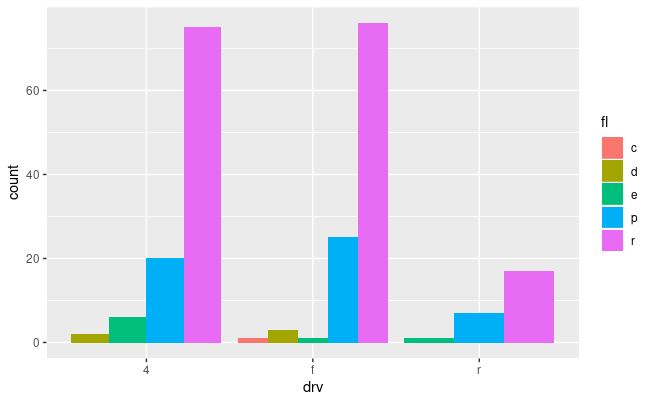
\includegraphics[width=\textwidth]{img/bivar-clustered-bar-chart}
    \caption{A clustered bar chart.}
    \label{fig:clustered-bar-chart}
  \end{subfigure}
  \begin{subfigure}{.33\textwidth}
    \centering
    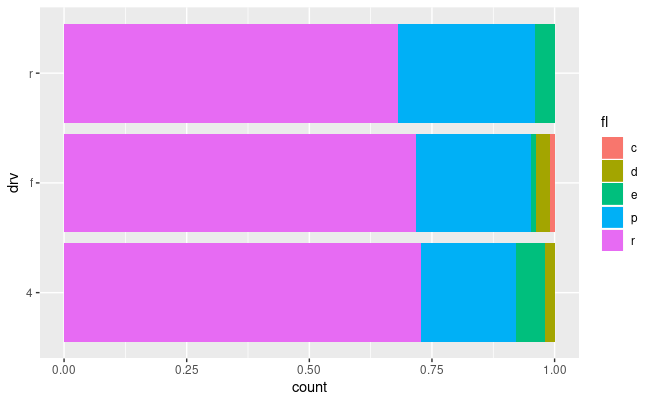
\includegraphics[width=\textwidth]{img/bivar-horizontal-stacked-bar-chart}
    \caption{A horizontal stacked bar chart.}
    \label{fig:stacked-bar-chart}
  \end{subfigure}
  \begin{subfigure}{.33\textwidth}
    \centering
    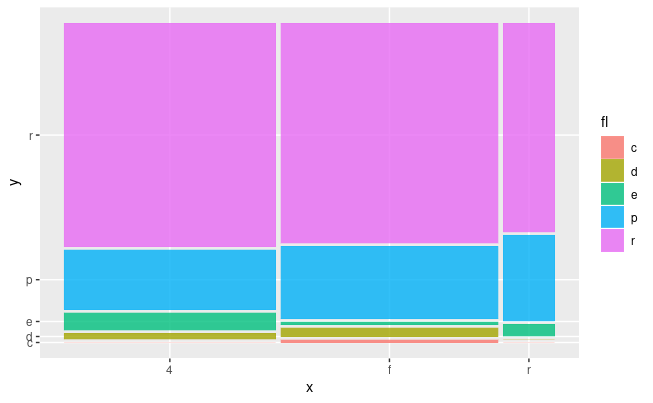
\includegraphics[width=\textwidth]{img/bivar-mosaic-plot}
    \caption{A mosaic plot.}
    \label{fig:mosaic-plot}
  \end{subfigure}
  \caption[Visualization techniques for 2 qualitative variables]{Visualization techniques for 2 qualitative variables. In all graph types the same data is presented.}
\end{figure}


\section{Qualitative-Quantitative}
\label{sec:qualitative-quantitative}

In this section we look at methods for determining a relationship between a qualitative (independent) variable and a quantitative (dependent) variable. A study of gender inequality in salaries in the ICT sector is a good example of this. The independent variable \emph{gender} is nominal (possible values could for example be M/F/X), the dependent variable \emph{gross salary} is a ratio variable.

The approach that is typically used is to compare the mean and/or standard deviation of the dependent variable between the different groups arising from the independent. If the differences are small, they can be attributed to random sampling errors and we conclude that there is no relationship. If the differences are large, we conclude that there \emph{is} a relationship. For example, it still is often the case that men earn significantly more than women for a similar job!

In this course we will discuss the $t$-test for 2 samples to determine if there is a difference between two groups (cfr. Section~ref{ssec:t-test-two-samples}). There exist statistical tests that extend this to a larger number of groups at the same time (e.g. the ANOVA-test), but these are out of scope for this syllabus.

As with Cramér'V for qualitative variables, there are also metrics that indicate the strength of the relationship between qualitative and a quantitative variables. In this context, these are often called the \emph{effect size}. In this syllabus we will investigate one metric for effect size, Cohen's $d$ (cfr. Section~\ref{ssec:cohens-d}). Again, there are multiple types of effect size, also suited for other measurement levels, but these are out of scope for this syllabus.

\subsection{The \texorpdfstring{$t$}{t}-test for two samples}
\label{ssec:t-test-two-samples}

The $t$-test introduced in Section~\ref{sec:t-test} can also be used to compare two samples. This way, you can determine if the difference between the sample mean of both samples is \emph{significantly} different.

A distinction is made between two cases:

\begin{itemize}
  \item Both samples are independent, taken separately. An example is a study on a medical treatment method in which a control group does \emph{not} receive the treatment and a test group does receive the treatment.
  \item The samples are dependent or paired. An example is taking two measurements on the same member of the population, for example measuring the fever before and after taking a certain drug to measure its effect.
\end{itemize}

In R you can also use the function \texttt{t.test} to conduct a test with two samples. We provide two examples below, one for each case.

\begin{example}
  In a clinical study, the aim is to determine whether a new drug has a delayed (i.e. higher) reaction speed as a side effect~\autocite{Lindquist}. 
  
  Six participants were given the drug (intervention group) and six others a placebo (control group). Next their response time to a stimulus was measured (in ms). We want to determine whether there are significant differences between the intervention and control groups.
  
  \textbf{Remark}: The intervention group and the control group happen to be the same size (6 test subjects for each).
  This is not necessary. For independent (unpaired) samples both groups may have a different size.
  
  \begin{itemize}
    \item Control group: 91, 87, 99, 77, 88, 91 ~~~~~~~~~~~~($\overline{x}=88,83$)
    \item Intervention group: 101, 110, 103, 93, 99, 104 ~~($\overline{y}=101,67$)
  \end{itemize}
  
  We note $\mu_1$ for the mean of the untreated population (control group) and $\mu_2$ for the population mean of patients who took the drug (intervention group).
  
  The hypotheses are formally noted as follows:
  
  $H_0: \mu_1 - \mu_2 = 0$ en $H_1: \mu_1 - \mu_2 < 0$
  
  As test statistic we use $\overline{x}-\overline{y}$, with $\overline{x}$ and $\overline{y}$ estimations for the \textit{real} values $\mu_1$ en $\mu_2$.

  Therefore, this is a left-tailed test, specified by the option \texttt{alternative = "less"}. For the null hypothesis, we assume that the difference between the population means is 0, indicated by the option \texttt{mu = 0}. Note that this is the default value for this parameter and therefore its value does not need to be specified in theory.

  \begin{lstlisting}
  control <-  c(91, 87, 99, 77, 88, 91)
  intervention <- c(101, 110, 103, 93, 99, 104)
  t.test(control, intervention, alternative="less", mu=0)
  \end{lstlisting}
  
  The result of the test:
  
  \begin{verbatim}
  t.test(control, intervention, alternative="less")
  
  Welch Two Sample t-test

  data:  control and intervention
  t = -3.4456, df = 9.4797, p-value = 0.003391
  alternative hypothesis: true difference in means is less than 0
  95 percent confidence interval:
  -Inf -6.044949
  sample estimates:
  mean of x mean of y 
  88.83333 101.66667 
  \end{verbatim}
  
  The test statistic $\overline{x}-\overline{y}=-12.833$ corresponds to a $t$-value $t=-3.4456$.
  The parameter $df=9.48$ is determined by \texttt{t.test()} based on the number of elements in the arrays $x$ and $y$.
  The calculation of this value is \textit{not} trivial.

  The $p$-value, 0.003391, is clearly below the significance level (not specified explicitly, so the default value $\alpha = 0.05$ was used).
  
  We can therefore reject the null hypothesis and conclude that, based on the results of this sample, the drug did have a significant effect on the reaction speed of patients.
  
  \textbf{Remark}: Because $\overline{x}-\overline{y}=-12.833$
  we can say with a confidence of 95\% that the difference of the \textit{real} means ($\mu_1-\mu_2$)
  of a larger control and intervention group will be between $-\infty$ en $-6.044949$.
  Cfr. Section~\ref{ssec:confidence-interval-pop-mean-large-sample} (p. \pageref{ssec:confidence-interval-pop-mean-large-sample})
  and \ref{ssec:confidence-interval-pop-mean-small-sample} (p. \pageref{ssec:confidence-interval-pop-mean-small-sample})
  regarding confidence intervals.
\end{example}


\begin{example}
  A study examined whether cars that run on petrol with additives have a lower consumption. Ten cars were first refueled with either regular petrol or petrol with additives (determined by flipping a coin), after which the consumption was measured (expressed in miles per gallon). The cars were then refueled with the other type of petrol and consumption was again measured. The results are given in the table below.
  
  \begin{center}
    \begin{tabular}{|l|c|c|c|c|c|c|c|c|c|c|}
      \hline 
      Car & 1 & 2 & 3 & 4 & 5 & 6 & 7 & 8 & 9 & 10 \\ 
      \hline 
      Regular petrol & 16 & 20 & 21 & 22 & 23 & 22 & 27 & 25 & 27 & 28 \\ 
      \hline 
      With additives & 19 & 22 & 24 & 24 & 25 & 25 & 25 & 26 & 28 & 32 \\ 
      \hline 
    \end{tabular} 
    %  \caption{Consumption in miles per gallon for 2 types of petrol.}
    %  \label{tab:petrol-consumption-additives}
  \end{center}
  
  We use a \emph {paired $t$-test} to determine whether cars run significantly more efficiently when using petrol with additives.
  
  We select $x$ for petrol \texttt{with additives} ($\overline{x}=25.1$ miles per gallon), and $y$ for \texttt{regular} petrol ($\overline{y}=23.1$ miles per gallon).
  
  The null hypothesis $H_0$ states that the miles per gallon is similar for both types ($\mu_{x-y}=0$).
  The alternative hypothesis $H_1$ states that you can drive a longer distance when using petrol with additives ($\mu_{x-y}>0$).
  
  The option \texttt{paired=TRUE} indicates that this is a paired $t$-test.
  
  \begin{lstlisting}
  regular <- c(16, 20, 21, 22, 23, 22, 27, 25, 27, 28)
  additives <- c(19, 22, 24, 24, 25, 25, 26, 26, 28, 32)
  t.test(additives, regular, alternative="greater", paired=TRUE)
  \end{lstlisting}
  
  Result:
  
  \begin{verbatim}
  Paired t-test
  
  data:  additives and regular
  t = 4.4721, df = 9, p-value = 0.0007749
  alternative hypothesis: true difference in means is greater than 0
  95 percent confidence interval:
  1.180207      Inf
  sample estimates:
  mean of the differences 
  2 
  \end{verbatim}
  
  The test statistic $\overline{x-y}=2$. This corresponds to a $t$-value of $t=4.4721$.
  The $p$-value, 0.0007749, is below the significance level ($\alpha=0.05$), so we can reject the null hypothesis. According to this sample, cars do drive more efficiently when using petrol with additives.
  
  \textbf{Remark}: For 95\% of the ``pairs'' from a larger population of cars, the difference $x-y$ will be located between $1.180207$ and $+\infty$.
  This is the confidence interval introduced in Section \ref{ssec:confidence-interval-pop-mean-large-sample} (p. \pageref{ssec:confidence-interval-pop-mean-large-sample})
  and \ref{ssec:confidence-interval-pop-mean-small-sample} (p. \pageref{ssec:confidence-interval-pop-mean-small-sample}).
\end{example}


\subsection{Effect Size - Cohen's \texorpdfstring{$d$}{d}}
\label{ssec:cohens-d}

The \emph{effect size}\index{effect size} is a metric that represents the impact (or effect) of an event. In most variants, a large value indicates a larger effect, whereas a value of 0 indicates the absence of an effect.

In this section, we introduce Cohen's $d$\index{Cohen's $d$}, developed by the American psychologist and statistician Jacob Cohen\index{Cohen, Jacob}. In particular, this metric is often used in publications on research into effects on learning outcomes in education. A study in this context is often set up as follows:

The researchers want to know the effect of a particular intervention on student learning. For example, they want to try out a new teaching method and determine whether it is suitable. Test subjects are selected who are typically randomly divided into two groups: a control group that gets to process a piece of learning material in a ``classic'' way and an intervention group that is presented with the same learning material using the new teaching method. After the class, a test is used to determine to what extent students of both groups have acquired the subject matter. We expect that students from the intervention group achieve a significantly better result than students from the control group. In scientific publications resulting from this type of research, the effect size will often be used.

John \textcite{Hattie2012}\index{Hattie, John} has been collecting publications on research in education for decades and maintains a list of effect sizes of all kinds of things that have an impact on student outcomes. This is not just about teaching methods, but also about student learning strategies, demographic factors (gender, social status, etc.), school and class management, etc. In his meta-analysis, most of the factors studied have a positive effect on learning outcomes, which may well be due to \emph{publication bias}. 

The average reported effect size is around $d = 0.4$. Hattie's recommendation therefore is that schools that want to have a positive effect on the learning outcomes of students should first look at factors that result in an effect size of at least 0.4. As a rule of thumb, you can say that an intervention with $d = 1$ means that the course material that is normally covered in one year can be processed in half the time. Table~\ref{table:effect-size} summarizes the interpretation of different values for Cohen's $d$.

\begin{definition}[Cohen's $d$]
  is defined as the difference between the two means divided by a standard deviation of the sample, or more concrete:
  \begin{equation}
  d = \frac{\overline{x}_1 - \overline{x}_2}{s}
  \end{equation}
  
  with $\overline{x}_1$ and $\overline{x}_2$ the mean of both groups and $s$ a combined standard deviation for two independent samples:
  
  \begin{equation}
  s = \sqrt{\frac{(n_1 - 1) s_1^2 + (n_2 - 1) s_2^2}{n_1 + n_2 - 2}}
  \end{equation}
  
  with $s_1^2$ and $s_2^2$ the sample variance of both groups and $n_1$ and $n_2$ the number of observations in each group (sample size).
\end{definition}

\begin{table}
  \centering
  \begin{tabular}{rl}
    \toprule
    \textbf{$|d|$} & \textbf{Effect Size} \\
    \midrule
    0.01 & Very small \\
    0.20 & Small \\
    0.50 & Average \\
    0.80 & Large \\
    1.20 & Very large \\
    2.00 & Huge \\
    \bottomrule
  \end{tabular}
  \caption{Interpretation of the absolute value of Cohen's $d$. Note that $d$ cam also be less than 0, indicating a negative effect of the intervention.}
  \label{table:effect-size}
\end{table}

\subsection{Visualization Techniques}
\label{ssec:qual-quant-visualization}

\subsubsection{Box Plot}

% TODO   Boxplot

\subsubsection{Bar chart with error bars}

% TODO  Staafdiagram met error bars

\section{Quantitative--Quantitative}

% TODO: inleiding
% TODO: Spreidingsdiagram

\subsection{Regression}
\label{sec:regression}

With regression\index{regression} we will try to find a consistent and systematic relationship between the variables. Or more concrete: ``if we know the value of the independent variable, can we predict the value of the dependent variable?'' There are two types of relationships:

\begin{description}
  \item [Monotonic:] a monotonic relationship is a relationship in which the researcher can indicate the general direction of the relationship between the two variables, either increasing or decreasing. The direction of the relationship never changes.
  \item[Non-monotonic:] in a non-monotonic relationship, the presence (or absence) of one variable is systematically related to the presence (or absence) of another variable. However, the direction of the relationship cannot be indicated.
\end{description}

In linear regression we will limit ourselves to a linear relationship: a linear relationship between an independent and dependent variable, where knowledge of the independent variable gives knowledge about the dependent variable.

In a linear relationship, there are three characteristics:

\begin{enumerate}
  \item Presence: is there a relationship between the two variables?
  \item Direction: is the relationship increasing or decreasing?
  \item What is the strength of the relationship: strong, moderate or nonexistent?
\end{enumerate}

An example of a linear relationship $y = \beta_{0} + \beta_{1}x$ can be found in Figure \ref{fig:regression-example}.

\begin{figure}[t]
  \begin{tikzpicture}
    \begin{axis}[
        axis x line=middle,
        axis y line=middle,
        enlarge y limits=true,
        width=\textwidth, height=8cm,     % size of the image
        grid = major,
        grid style={dashed, gray!30},
        ylabel=$y$,
        xlabel=$x$,
        legend style={at={(0.1,-0.1)}, anchor=north}
      ]
      \addplot[only marks] table  {data/regression.dat};
      \addplot [no markers, thick, red] table [y={create col/linear regression={y=y}}] {data/regression.dat};
    \end{axis}
  \end{tikzpicture}
  \caption{Example of a linear relationship}
  \label{fig:regression-example}
\end{figure}

We can find such a relationship using Gauss's \index{method of least squares} method of least squares. This is done as follows.

\begin{theorem}

  A linear relationship is represented as follows:

  \begin{equation}
    y = \beta_{0} + \beta_{1} x
    \label{eq:lineair}
  \end{equation}
  with
  \begin{itemize}
    \item $y$ the dependent
    \item $x$ the independent
  \end{itemize}

  We want to minimalize the squared sum of the deviations $e_{i} = y_{i} - (\beta_{0} + \beta_{1}x_{i})$. Such a deviation can also be formulated as (assume $X_{i} = x_{i} - \overline{x}$ and $Y_{i} = y_{i} - \overline{y}$):

  \begin{eqnarray}
    e_{i} & = & y_{i} - \beta_{1} x_{i} - \beta_{0} \\
    e_{i} & = & (y_{i} - \overline{y}) - \beta_{1}(x_{i} - \overline{x}) - (\beta_{0} - \overline{y} + \beta_{1} \overline{x}) \\
    \label{eq:regression-proof}
    e_{i} & = & Y_{i} - \beta_{1} X_{i} - (\beta_{0} - \overline{y} + \beta_{1} \overline{x})
  \end{eqnarray}

  In step~\ref{eq:regression-proof} we actually calculate $+\overline{x}-\overline{x}+\overline{y}-\overline{y}$, which is a null operation. This step is not so obvious, but remember that this is a ``shortcut'' to the solution, and that the ``real'' proof is a lot more complicated.

  We want to minimimalize the squared sum $e_i$:

  \begin{eqnarray}
    \sum_{i}^{n} e_{i}^{2} & =& \sum_{i}^{n} (y_{i} - (\beta_{0} + \beta_{1}x_{i}))^{2}\\
    & = & \sum_{i}^{n} ((Y_{i} - \beta_{1} X_{i}) - (\beta_{0} - \overline{y} + \beta_{1}\overline{x}))^{2}\\
    & = & \sum_{i}^{n}(Y_{i} - \beta_{1} X_{i})^2 - 2 \sum_{i}^{n}(Y_i - \beta_1 X_i)(\beta_0 - \overline{y}+ \beta_1\overline{x}) + \sum_{i}^{n}(\beta_{0} - \overline{y} + \beta_{1}\overline{x})^{2} \label{eq:step1}\\
    & = & \sum_{i}^{n}(Y_{i} - \beta_{1} X_{i})^{2} + n(\beta_{0} - \overline{y} + \beta_{1} \overline{x})^{2} \label{eq:step2}
  \end{eqnarray}

  We can go from \ref{eq:step1} to \ref{eq:step2} as follows:

  \[ \sum_{i}^{n}X_i = \sum_{i}^{n} (x_i - \overline{x}) = 0 \]
  and equivalent
  \[ \sum_{i}^{n}Y_i = \sum_{i}^{n} (y_i - \overline{y}) = 0 \]
  therefore
  \[ \sum_{i}^{n}(Y_i - \beta_1 X_i) = \sum_{i}^{n}Y_i - \beta_1 \sum_{i}^{n}X_i = 0 \]
  and also
  \[ 2 \sum_{i}^{n}(Y_i - \beta_1 X_i)(\beta_0 - \overline{y}) \]
  

  Now $e^{2}_{i}$ is written as a sum of two positive expressions. This sum is minimal if both expressions are minimal.

  \begin{equation}
    \begin{cases}
      \sum_{i}^{n}( Y_{i} - \beta_{1} X_{i})^{2} \textnormal{ is minimal.}\\
      n(\beta_{0} - \overline{y} + \beta_{1} \overline{x})^{2} \textnormal{ is minimal}
    \end{cases}
    \label{eq:vgl}
  \end{equation}


  For the first expression we actually find a quadratic function in $\beta_1$.
  \begin{eqnarray}
		& \sum_{i}^{n}( Y_{i} - \beta_{1} X_{i})^{2} \textnormal{ is minimal.} \label{eq:expression}\\
		\Leftrightarrow & \sum_i^n (Y_i^2 - 2X_iY_i\beta_1 + X_i^2\beta_1^2) \textnormal{ is minimal.} \\
		\Leftrightarrow & \beta_1^2 \sum_i^n X_i^2 - 2\beta_1 \sum_i^n X_iY_i + \sum_i^nY_i^2 \textnormal{ is minimal.} \\
		\Leftrightarrow & \textnormal{is minimal if } \beta_{1} = \frac{\sum_{i}^{n} X_{i}Y_{i}}{\sum_{i}^{n} X_{i}^{2}}
  \end{eqnarray}
  
  For the second expression we have that

  \begin{eqnarray}
		& n(\beta_{0} - \overline{y} + \beta_{1} \overline{x})^{2} \textnormal{ is minimal}
		\Leftrightarrow & n(\beta_{0} - \overline{y} + \beta_{1} \overline{x})^{2} = 0 \\
		\Leftrightarrow & \beta_{0} - \overline{y} + \beta_{1} \overline{x} = 0 \\
		\Leftrightarrow & \beta_{0} = \overline{y} - \beta_{1}\overline{x} 
  \end{eqnarray}
  

  with solution

  \begin{equation}
    \begin{cases}
      \beta_{1} = \frac{\sum_{i}^{n} X_{i}Y_{i}}{\sum_{i}^{n} X_{i}^{2}}\\
      \beta_{0} = \overline{y} - \beta_{1}\overline{x}
    \end{cases}
    \label{eq:vgl2}
  \end{equation}

  and therefore

  \begin{eqnarray}
    \beta_{1} & = & \frac{\sum_{i}^{n} (x_{i} - \overline{x})(y_{i} - \overline{y})}{\sum_{i}^{n} (x_{i} - \overline{x})^{2}} \\
    \beta_{0} & = & \overline{y} - \beta_{1} \overline{x}
    \label{eq:regressie}
  \end{eqnarray}
\end{theorem}


\begin{table} \centering
  \begin{tabular}{@{}rr@{}} \toprule
    Protein content\%& Weight gain (grams)  \\
    \midrule
    0		&	177 \\
    10 	&	231	\\
    20	& 249	\\
    30	& 348 \\
    40	& 361 \\
    50	& 384 \\
    60	& 404 \\
    \bottomrule
  \end{tabular}
  \caption{The data collected by Santa Claus: weight gain per protein percentage is considered.}
  \label{tab:reindeer}
\end{table}



\begin{table} \centering
  \begin{tabular}{@{}llllll@{}}
    \toprule
    $x$   & $y$     & $x-\overline{x}$    & $y - \overline{y}$        & $(x-\overline{x})(y - \overline{y})$       &  $(x-\overline{x})^{2}$    \\ \midrule
    0  & 177 & -30 & -130,71 & 3921,3 & 900  \\
    10 & 231 & -20 & -76,71  & 1534,2 & 400  \\
    20 & 249 & -10 & -58,71  & 587,1  & 100  \\
    30 & 348 & 0   & 40,29   & 0      & 0    \\
    40 & 361 & 10  & 53,29   & 532,9  & 100  \\
    50 & 384 & 20  & 76,29   & 1525,8 & 400  \\
    60 & 404 & 30  & 96,29   & 2888,7 & 900  \\
    &     &     &         & 10990  & 2800 \\ \bottomrule
  \end{tabular}
  \caption{Calculations required to apply the method of least squares.}
  \label{tab:reindeer2}
\end{table}

\begin{figure}
  \begin{tikzpicture}
    \begin{axis}[
        axis x line=middle,
        axis y line=middle,
        enlarge y limits=true,
        width=\textwidth, height=8cm,     % size of the image
        grid = major,
        grid style={dashed, gray!30},
        ylabel=weight gain (g),
        xlabel=protein content (\%),
        legend style={at={(0.1,-0.1)}, anchor=north}
      ]
      \addplot[only marks] table  {data/santa.txt};
      \addplot [no markers, thick, red] table [y={create col/linear regression={y=y}}] {data/santa.txt};
    \end{axis}
  \end{tikzpicture}

  \caption{Linear relationship between protein content and weight gain}
  \label{fig:reindeerFigure}
\end{figure}

\begin{example}
  \label{ex:reindeer}
  We look at the example of Santa Claus and his reindeer. He wants to find out if there is a linear relationship between the protein content of the food and the weight gain of the reindeer. He performs a number of experiments and obtains the data of Table \ref{tab:reindeer}. By applying the formulas above, we have that (see Table \ref{tab:reindeer2}):
  \[ \beta_{1} = \frac{\sum_{i=1}^{n} (x_{i}-\overline{x})(y_{i} - \overline{y})}{\sum_{i=1}^{n} (x_{i}-\overline{x})^{2}} = \frac{10990}{2800} = 3.925 \]
  \[ \beta_{0} = \overline{y} - \beta_{1} \overline{x} = 307.7143 - 3.925 \times 30 = 189.96 \]
  Thus, a linear relationship has been found which minimizes the squares of the residues. However, note that nothing is being said about the strength or validity of this relationship. This relationship is drawn in Figure \ref{fig:reindeerFigure}.
\end{example}

Example~\ref{ex:reindeer} solved in R (including a plot of the regression line):

\lstinputlisting{data/regression.R}

\subsection{Correlation}
\label{sec:correlation}

\subsection{Pearson product-moment correlation coefficient}

We can determine two statistics that express the strength of a linear relationship. These are also---just like the $\chi^2$-test---developed by Karl Pearson\index{Pearson!Karl}.

\begin{definition}[Pearson product-moment correlation coefficient]
  The Pearson product-moment correlation coefficient\index{Pearson product-moment correlation coefficient} $R$ (or in short the correlation coefficient\index{correlation coefficient}) is a measure for the strength of a linear correlation between two variables X and Y. It has a value between -1 and 1.
  
  \begin{itemize}
    \item A value of +1 indicates a (total) positive linear correlation.
    \item A value of -1 indicates a (total) negative linear correlation.
    \item A value of 0 indicates that there is no linear correlation.
  \end{itemize}
  
  The closer the correlation coefficient is to 1 or -1, the better the quality of the linear model.
\end{definition}

\subsubsection{Coefficient of determination}

\begin{definition}
  The \index{Coefficient of determination}coefficient of determination ($R^{2}$) is the square of the correlation coefficient and explains the percentage of the variance of the observed values relative to the regression line.

  \begin{itemize}
    \item $R^{2}$ is the explained variance
    \item $1-R^{2}$ is the unexplained variance
  \end{itemize}
\end{definition}

\begin{figure}[t]
  \begin{tikzpicture}
    \begin{axis}[
        axis x line=middle,
        axis y line=middle,
        enlarge y limits=true,
        width=\textwidth, height=8cm,     % size of the image
        grid = major,
        grid style={dashed, gray!30},
        ylabel=family size mother,
        xlabel=family size,
        legend style={at={(0.1,-0.1)}, anchor=north}
      ]
      \addplot[only marks] table  {data/families.txt};
      \addplot [no markers, thick, red] table [y={create col/linear regression={y=y}}] {data/families.txt};
    \end{axis}
  \end{tikzpicture}
  \caption{Linear relationship between the size of a family and the size of the family of the mother}
  \label{fig:motherRelationship}
\end{figure}

\tikzset{small dot/.style={fill=black, circle,scale=0.2}}
\tikzset{every pin/.style={draw=black,fill=yellow!10}}

\begin{figure}[t]%
  \begin{tikzpicture}
    \begin{axis}[
        axis x line=middle,
        axis y line=middle,
        enlarge y limits=true,
        width=\textwidth, height=8cm,     % size of the image
        grid = major,
        grid style={dashed, gray!30},
        ylabel=family size mother,
        xlabel=family size,
        legend style={at={(0.1,-0.1)}, anchor=north}
      ]
      \draw (axis cs:3,0)--(axis cs:3,8);
      \draw (axis cs:0,4.3)--(axis cs:6,4.3);
      \node[small dot, pin=120:{$III$}] at (axis cs:1.6,7) {};
      \node[small dot, pin=120:{$I$}] at (axis cs:5.5,7) {};
      \node[small dot, pin=120:{$II$}] at (axis cs:1.6,2) {};
      \node[small dot, pin=120:{$IV$}] at (axis cs:5.5,2) {};
      \addplot[only marks] table  {data/families.txt};
    \end{axis}
  \end{tikzpicture}
  \caption{The figure divided into 4 quadrants}%
  \label{fig:quadrants}%
\end{figure}

\subsubsection{Determination of $R$ and $R^{2}$}
\label{sec:determination-coefficient}
Consider the example of Figure \ref{fig:motherRelationship}: the size of a family vs. the size of the mother's family. We clearly see that there is a linear relationship. If we calculate the mean and divide the figure into 4 quadrants (quadrant $I$, $II$, $III$, $IV$) according to the means we get the figure of \ref{fig:quadrants}. We can then investigate the following situations.

\begin{itemize}
  \item Consider an element from area I. For this element $x_{i} - \overline{x}$ is positive and $y_{i} - \overline{y}$ also. Therefore the product $(x_{i} - \overline{x}) (y_{i} - \overline{y}) > 0$.
  \item Consider an element from area II. For this element $x_{i} - \overline{x}$ is negative and $y_{i} - \overline{y}$ also. Therefore the product $(x_{i} - \overline{x}) (y_{i} - \overline{y}) > 0$.
  \item Consider an element from area III. For this element $x_{i} - \overline{x}$  is negative and $y_{i} - \overline{y}$ positive. Therefore the product $(x_{i} - \overline{x}) (y_{i} - \overline{y}) < 0$.
  \item Consider an element from area IV. For this element $x_{i} - \overline{x}$ is positive and $y_{i} - \overline{y}$ negative. Therefore the product $(x_{i} - \overline{x}) (y_{i} - \overline{y}) < 0$.
\end{itemize}

Since there are more points in areas I and II than there are in areas III and IV, the sum $\sum_{i} (x_{i} - \overline{x}) (y_{i} - \overline{y})$ will be a positive number. The more points there are in areas I and II, the larger the number will be. We therefore notice a strong positive linear relationship.

If the points were evenly distributed over the four areas, we have that the value will sometimes be close to zero. On the other hand, if there is a negative linear relationship, we will have a negative number.

We therefore found a measure for the relationship between two variables:

\begin{itemize}
  \item For increasing correlated relationships  $\sum_{i} (x_{i} - \overline{x}) (y_{i} - \overline{y})$ is positive and large.
  \item For decreasing correlated relationships $\sum_{i} (x_{i} - \overline{x}) (y_{i} - \overline{y})$ is negative and large (in absolute value).
  \item For uncorrelated variables $\sum_{i} (x_{i} - \overline{x}) (y_{i} - \overline{y})$ is small in absolute value.
\end{itemize}

We can make this measure independent of the size of the sample by dividing it by the sample size $n$. This is called the co-variance and is defined as a common distribution:

\begin{equation}
  Cov(X,Y) = \frac{\sum_{i}^{n}(x_{i} - \overline{x}) (y_{i} - \overline{y})}{n - 1}
  \label{eq:covariance}
\end{equation}

This gives us the average deviation per measuring point.

Note that for the covariance, similar to the variance, a distinction is made between the covariance of a population (denominator $n$) and a sample (denominator $n-1$). In practice you assume that you are dealing with a sample, so you will usually use the formula with $n-1$ in the denominator. The R-function \texttt{cov()} also uses this definition.

To normalize again (a variation in X is not necessarily of the same magnitude as a variation in Y) we will make the criteria for the combined variation independent of the number of observations and the order of magnitude of the numeric values. This way we can make these values universally comparable. To do so, we divide the covariance by the product of the standard deviations, and we call this the relative covariance or the  Pearson correlation coefficient als known as the product-moment correlation coefficient or in short correlation coefficient.

\begin{align}
  R &=\frac{COV(X,Y)}{\sigma_{x}\sigma_{y}} \\
    &= \frac{COV(X,Y)}{\sqrt{\frac{\sum(x_{i} - \overline{x})^{2}}{n-1}} \times \sqrt{\frac{\sum(y_{i} - \overline{y})^{2}}{n-1}}} \\
    &= \frac{\sum_{i}^{n}(x_{i}-\overline{x})(y_{i} - \overline{y})}{\sqrt{\sum_{i}^{n} (x_{i}-\overline{x})^{2}} \sqrt{\sum_{i}^{n} (y_{i}-\overline{y})^{2}}}
  \label{eq:relative-covariance}
\end{align}

The correlation coefficient is independent of the unit of measurement whereas the covariance is dependent on the unit of measurement.

\subsubsection{Interpretation of $R^{2}$}

If we assume that $x$ does not contribute to the prediction of $y$, the best prediction of a value of $y$ is the sample mean $\overline{y}$, illustrated in Figure \ref{fig:reindeerFigure3} as a horizontal line. The vertical line segments are the deviations from the observed points $y$ from this prediction (the sample mean). The squared sum of these deviations is:

\[ SS_{yy} = \sum(y_{i} - \overline{y})^{2} \]

If we assume that $x$ does play a role in the prediction of $y$, we calculate the regression line for the same data set and the deviations of the points from the line as illustrated in Figure \ref{fig:reindeerFigure2}.

\[ SSE_{yy} = \sum(y_{i} - \widehat{y})^{2} \]

If we now compare the deviations with each other, we see the following:
\begin{enumerate}
  \item If $x$ contributes little or not at all to the prediction, the squared sum of the deviations of the two lines will be almost identical:
    \[ SS_{yy} = \sum(y_{i} - \overline{y})^{2} \] and
    \[ SSE_{yy} = \sum(y_{i} - \widehat{y})^{2} \]
    in which $\widehat{y}$ is the predicted value. 
  \item If $x$ does contribute to the prediction of $y$, $SSE_{yy}$ will be smaller than $SS_{yy}$. In fact,
    \[	SSE_{yy} = \sum(y_{i} - \widehat{y})^{2} \]
    equals zero if all points are predicted perfectly (and therefore are located on regression line).
\end{enumerate}

The decrease in the squared sum that can be attributed to the inclusion of $x$ in the model is then (expressed as a fraction of $SS_{yy}$)
\[ \frac{SS_{yy} - SSE_{yy}}{SS_{yy}} \]
We call $SS_{yy}$ the total sample variance of the measurements around the sample mean $\overline{y}$ and $SSE_{yy}$ the remaining unexplained sample variance, after estimating the line $\widehat{y} = \beta_{0} + \beta_{1}x$. So $(SS_{yy} - SSE_{yy})$ is the explained variation due to the linear relationship with $x$.

It is now possible to illustrate that with simple linear regression this fraction 
\[ \frac{SS_{yy} - SSE_{yy}}{SS_{yy}} = \frac{\textnormal{explained variance}}{\textnormal{total sample variance}} \]
is equal to the square of the Pearson correlation coefficient. (= the part of the total variance explained by the linear line).

Table~\ref{tab:interpretation-correlation-coefficient} provides an overview of how the values of $R$ and $R^2$ can be interpreted, and in particular how strong the relationship between two variables is.

\begin{figure}
  \begin{tikzpicture}
    \begin{axis}[
        axis x line=middle,
        axis y line=middle,
        enlarge y limits=true,
        width=\textwidth, height=8cm,     % size of the image
        grid = major,
        grid style={dashed, gray!30},
        ylabel=protein content,
        xlabel=weight gain (g),
        legend style={at={(0.1,-0.1)}, anchor=north}
      ]
      \addplot[only marks] table  {data/santa.txt};
      \addplot [no markers, thick, red] table [y={create col/linear regression={y=y}}] {data/santa.txt};
      \addplot [mark=none, color=red] coordinates {
        (0,177) (0,189.9643)
      };
      \addplot [mark=none, color=red] coordinates {
        (10,231) (10,229.2143)
      };
      \addplot [mark=none, color=red] coordinates {
        (20,249) (20,268.4643)
      };
      \addplot [mark=none, color=red] coordinates {
        (30,348) (30,307.7143)
      };
      \addplot [mark=none, color=red] coordinates {
        (40,361) (40,346.9643)
      };
      \addplot [mark=none, color=red] coordinates {
        (50,384) (50,386.2143)
      };
      \addplot [mark=none, color=red] coordinates {
        (60,404) (60,425.4643)
      };

    \end{axis}
  \end{tikzpicture}
  \caption{Deviations from the regression line: assumption that $x$ provides additional information for predicting $y$.}
	\label{fig:reindeerFigure2}
\end{figure}

\begin{figure}
  \begin{tikzpicture}
    \begin{axis}[
        axis x line=middle,
        axis y line=middle,
        enlarge y limits=true,
        width=\textwidth, height=8cm,     % size of the image
        grid = major,
        grid style={dashed, gray!30},
        ylabel=protein content,
        xlabel=weight gain (g),
      ]
      \addplot[only marks] table  {data/santa.txt};
      \addplot [mark=none, color=black] coordinates {
        (0,307.71) (60,307.71)
      };
      \addplot [mark=none, color=red] coordinates {
        (0,177) (0,307.71)
      };
      \addplot [mark=none, color=red] coordinates {
        (10,231) (10,307.71)
      };
      \addplot [mark=none, color=red] coordinates {
        (20,249) (20,307.71)
      };
      \addplot [mark=none, color=red] coordinates {
        (30,348) (30,307.71)
      };
      \addplot [mark=none, color=red] coordinates {
        (40,361) (40,307.71)
      };
      \addplot [mark=none, color=red] coordinates {
        (50,384) (50,307.71)
      };
      \addplot [mark=none, color=red] coordinates {
        (60,404) (60,307.71)
      };

    \end{axis}
  \end{tikzpicture}
  \caption{Deviations from the mean of y: assumption that $x$ provides no information for predicting $y$ ($\overline{y} =307.71$).}
  \label{fig:reindeerFigure3}
\end{figure}

\begin{table} \centering \small
  \begin{tabular}{@{}rrrl} \toprule
    $|R|$ & $R^{2}$ & Explained variance &  Interpretation \\
    \midrule
    $< 0.3$       & $< 0.1$       & $< 10\%$    & very weak \\
    $0.3 - 0.5$   & $0.1 - 0.25$ & $10 - 25\%$  & weak \\
    $0.5 - 0.7$   & $0.25 - 0.5$  & $25 - 50\%$ & moderate \\
    $0.7 - 0.85$  & $0.5 - 0.75$  & $50 - 75\%$ & strong\\
    $0.85 - 0.95$ & $0.75 - 0.9$  & $75 - 90\%$ & very strong\\
    $> 0.95$      & $> 0.9$       & $>90\%$     & exceptional(!)\\
    \bottomrule
  \end{tabular}
  \caption[Interpretation of $R$ and $R^2$.]{Interpretation of $R$ and $R^2$.}
  \label{tab:interpretation-correlation-coefficient}
\end{table}

\section{Conclusion}

Different types of relationships between variables exist. We are mainly interested in monotonic and linear relationships. For this we have the correlation coefficient and linear regression. These techniques should not be used with nominal and ordinal variables. A small value $(=0)$ for a measure for the relationship only means that the corresponding relationship is absent: there can be a different type of relationship. It is therefore always recommended to use a scatter plot.

The fact that two variables are correlated does not mean that one is the cause of the other.

\section{Summary}

In this chapter, several techniques have been proposed to determine whether there is a relationship between two variables. One variable is called the \emph{independent}, the other is called the \emph{dependent} variable. We want to find out whether the value of the independent variable has an impact on the value of the dependent.

The techniques we can use (either arithmetic or for visualization) depend on the measurement level of the variables examined. Table~\ref{tab:overview-2-variables} provides an overview.

\begin{table}

  \begin{tabular}{llll}
    \toprule
    \multicolumn{2}{c}{\textbf{Measurement level variable}}             & \textbf{}                   & \textbf{}                                             \\
    \textbf{Independent}       & \textbf{Dependent}         & \textbf{Arithmetic}           & \textbf{Visualization}                                 \\
    \midrule
    \multirow{3}{*}{Qualitative}  & \multirow{3}{*}{Qualitative}  & $\chi^2$                    & mosaic plot                                        \\
    &                               & Cramér's V                  & clustered bar chart                               \\
    &                               &                             & horizontal stacked bar chart                                          \\
    \midrule
    \multirow{2}{*}{Qualitative}  & \multirow{2}{*}{Quantitative} & t-test for 2 samples & boxplot                                               \\
    &                               &                             & \parbox{4.5cm}{(alternatively bar graph mean with standard deviation)} \\
    \midrule
    \multirow{3}{*}{Quantitative} & \multirow{3}{*}{Quantitative} & covariance                 & scatter (XY) plot \\
    &                               & correlation coefficient       & regression line                                       \\
    &                               & coefficient of determination  &                                                      \\
    \bottomrule
  \end{tabular}
  
  \caption{Overview of techniques for the analysis of two variables.}
  \label{tab:overview-2-variables}
\end{table}

\section{Exercises}
\label{sec:bivariate-analysis-exercises}

The data files for these exercises can be found on Github under \emph{exercises/datasets}

\subsection{Qualitative--Qualitative}
\label{ssec:ex-qualitative-qualitative}

\begin{exercise}
  \label{ex:music-wine-analysis} % $\chi^{2}$ - manual}
  
  Market research suggests that background music in a supermarket has an influence on the behaviour of customers. In a study by~\textcite{Ryan1998}, three situations were compared: no music, French chansons, and Italian hits. In every case, the sales of French, Italian and other wine was recorded.
  
  The results of this study can be found in \emph{MusicWine.csv}. 
  
  Questions:
  \begin{enumerate}
    \item Generate a cross table (contingency table) for this study using R's \texttt{table} function to obtain the frequency table.
    \item Calculate marginal totals (column and row sums).
    \item Determine the expected values (e).
    \item Calculate the value of $\chi^{2}$ manually, including all intermediate values. Check your result by comparing with the result of the appropriate R-function for calculating $\chi^{2}$.
    \item Calculate Cramér's V manually. What can you conclude from its value?
  \end{enumerate}
\end{exercise}

\begin{exercise}
  \label{ex:ex:music-wine-crosstable-visualization}
  Visualise the data from Exercise~\ref{ex:music-wine-analysis} using the appropriate charts:
  \begin{enumerate}
    \item Plot the percentages of sold wines where \emph{Music} equals \emph{None} using a bar chart.
    \item Plot the same data using a clustered bar chart.
    \item Finally, plot the same dat ausing a horizontal stacked bar chart.
  \end{enumerate}
\end{exercise}

\begin{exercise}
  \label{ex:earthquakes} %$\chi^{2}$ in R}
  Import the data file \emph{earthquakes.csv} in R.
  \begin{enumerate}
    \item Plot a histogram and a box plot of the variable \emph{Magnitudes}.
    \item Plot a line graph with the number of recorded earthquakes per month.
    \item Determine wether there is a relationship between the variables \emph{Type} and \emph{Source}. Also calculate Cramér's V. What is the conclusion?
  \end{enumerate}
\end{exercise}

\begin{exercise}
  \label{ex:chisq-survey}
  For this exercise we will use the dataset \texttt{survey} that is included in R. This dataset consists of a survey among students. The dataset can be imported as follows:
  
  \begin{lstlisting}
  library(MASS)
  View(survey)  # Shows the "survey" dataset
  ?survey       # Help-page with explanation on the contents
  \end{lstlisting}
  
  If you get an error message when importing the library (first line), this means that the package \texttt{MASS} is not installed yet. You can fix this by selecting Tools > Install Packages and entering the package name in the text box.
  
  We want to investigate the relationship between some discrete (nominal or ordinal) variables in this dataset. For each of the pairs listed below, follow these steps:
  
  \begin{enumerate}[label=(\alph*)]
    \item First think about what outcome you expect for the given combination of variables.
    \item Compose a frequency table for the two variables. The (suspected) independent variable comes first.
    \item Plot a graph of the data, e.g. a clustered bar chart, stacked bar chart of the relative frequencies, or a ``mosaic plot'' (straightforward with \texttt{plot(table(data\$col1, data\$col2))}).
    \item If you look the graph, do you expect a large or a small value for the $\chi^2$ statistic? why?
    \item Calculate the $\chi^2$ statistic and the critical value $g$ (for a significance level $\alpha = 0.05$)
    \item Calculate the $p$-value
    \item Do we have to accept or reject the null hypothesis? What does this imply for the relationship between the two variables?
  \end{enumerate}
  
  The variables to be investigated are listed below. The suspected independent variable is always mentioned first.
  
  \begin{enumerate}
    \item \texttt{Exer} (exercising) and \texttt{Smoke} (smoking behavior)
    \item \texttt{W.Hnd} (writing hand) and \texttt{Fold} (the upper hand when crossing your arms)
    \item \texttt{Sex} (gender) en \texttt{Smoke}
    \item \texttt{Sex} en \texttt{W.Hnd}
  \end{enumerate}
\end{exercise}

\begin{exercise}
  \label{ex:chisq-aids2}
  Import the dataset \texttt{Aids2} from the package \texttt{MASS} (cfr. Exercise~\ref{ex:chisq-survey}) that contains information on 2,843 patients infected with AIDS in Australia before 1991. This dataset was discussed in detail by~\textcite{Ripley2007}. Investigate whether there is a relationship between the variable (\texttt{Sex}) and the category of contamination (\texttt{T.categ}).
  
  \begin{enumerate}
    \item Proceed in the usual way: visualize the data, calculate $\chi^2$, $g$ and $p$-value ($\alpha = 0,05$), and finally formulate a conclusion.
    \item Calculate the standardized residuals to determine which categories contain extreme values.
  \end{enumerate}
  
\end{exercise}

\begin{exercise}
  \label{ex:chisq-digimeter}
  
  Every year Imec (formerly iMinds) conducts a study on the use of digital technologies in Flanders, the Digimeter~\autocite{Vanhaelewyn2016}. In this exercise we will determine whether the sample used by the Digimeter 2016 ($n = 2164$) is representative of the population in terms of the age categories of the participants.
  
  Table~\ref{tab:digimeter2016} shows the relative frequencies of the participants. The absolute frequencies for the different age categories of the Flemish population are summarized in Table~\ref{tab:age-Flanders}. This information can also be found in the attached CSV file \texttt{oefeningen/data/bestat-vl-ages.csv}.
  
  \begin{enumerate}
    \item The table with age data of the Flemish population as a whole has more categories than those used by the Digimeter. Make a summary of this table so that you have the same categories as the Digimeter. Tip: this may be easier to do in a spreadsheet than in R.
    \item In order to apply the goodness of fit test, we need the absolute frequencies of the observed values in the sample. Calculate this.
    \item Also calculate the expected percentages ($\pi_{i}$) for the population as a whole.
    \item Apply the goodness of fit test on the distribution of age categories in the sample used by the Digimeter. Is the sample representative for the Flemish population in this respect?
  \end{enumerate}
\end{exercise}

\begin{table}
  \caption{Frequencies of the age of participants in the iMec Digimeter 2016 and the Flemish population.}
  \label{tab:frequenties-leeftijden}
  \centering
  \begin{tabular}{cc}
    \textbf{Age Group} & \textbf{Percentage} \\ \midrule
    15-19 & 6,6\% \\
    20-29 & 14,2\% \\
    30-39 & 15,0\% \\
    40-49 & 16,3\% \\
    50-59 & 17,3\% \\
    60-64 & 7,3\% \\
    64+   & 23,2\% \\
  \end{tabular}
  \subcaption{Percentage of participants in iMec's Digimeter 2016 ($n = 2164$), broken down by age range. \autocite{Vanhaelewyn2016}}
  \label{tab:digimeter2016}
  
  \centering
  \begin{tabular}{cc}
    \textbf{Age Group} & \textbf{Count} \\ \midrule
    –5            &     352017      \\
    5-9           &     330320      \\
    10-14          &     341303      \\
    15-19          &     366648      \\
    20-24          &     375469      \\
    25-29          &     387131      \\
    30-34          &     401285      \\
    35-39          &     409587      \\
    40-44          &     458485      \\
    45-49          &     493720      \\
    50-54          &     463668      \\
    55-59          &     413315      \\
    60-64          &     379301      \\
    65-69          &     299152      \\
    70-74          &     279789      \\
    75-79          &     249260      \\
    80-84          &     182352      \\
    85-89          &     104449      \\
    90-94          &      29888      \\
    95-99          &      7678       \\
    100+           &       923
  \end{tabular}
  \subcaption{Absolute frequency of the Flemish population by age category. Source: BelStat (\url{https://bestat.economie.fgov.be/bestat/}, C01.1: Population by residence (province), gender, household position (C), marital status and age (B)).}
  \label{tab:age-Flanders}
    
\end{table}

\subsection{Qualitative--Quantitative}
\label{ssec:ex-qualitative-quantitative}

\begin{exercise}
  \label{ex:casus-akin2016-toets}
  
  In Exercise~\ref{oef:casus-akin2016-1var} and the subsequent exercises, we analyzed the results of performance measurements for persistence capabilities on Android~\autocite{Akin2016}. Experiments were performed for different combinations of data size (small, medium, large) and persistence type (GreenDAO, Realm, SharedPreferences, SQLite). For each data size, we were able to determine which persistence type yielded the best results. 
  
  Now we will find out if the best persistence type at first glance is also \emph{significantly} better than the competition.
  
  In concrete: Using a two-sample test for each data size, verify that the mean of the highest scoring persistence type is \emph{significantly lower} than the mean of the \emph{second} best and the worst scoring type.
  
  Can we maintain the conclusion that for a given data size, one persistence type is best, i.e. is significantly better than any other persistence type?
\end{exercise}

\begin{exercise}
  A large number of students participated in a test that was organized in several successive sessions. Because creating a separate test for each session was practically unfeasible, the same questions were used each time. In fact, there is a danger that students could pass on information about the test to the groups that still had to come after. Later groups then have an advantage over the first. Is this also evident from the figures?
  
  The file \texttt{puntenlijst.csv} contains all results of the test. Each group is identified by a letter, in the order of the session.
  
  \begin{itemize}
    \item Day 1: sessions A, B
    \item Day 2: sessions C, D, E
    \item Day 3: sessions F, G, H
  \end{itemize}
  
  Sessions A and B were conducted on a different campus, so it could be assumed that there is little to no communication with students from other sessions.
  
  If information was passed on successfully, we expect the scores of later groups to be significantly better than the first.
  
  Note that the reverse reasoning does not necessarily hold: if it turns out that the result of later sessions is indeed significantly better, this does not necessarily mean that the (only) cause is passing on of information. There may also be other causes (e.g. ``weaker'' class groups happen to be scheduled earlier).

  \begin{enumerate}
    \item Explore the data. Calculate the appropriate measures for central tendency and dispersion for the full dataset and for each session individually.
    
    \item Plot a bar graph of the average score per session. Is this sufficient to visualize the results? Why (not)?
    
    \item Make a box plot of the scores divided per group. Compare the sessions listed below. Do you think there is a significant difference between the results? Can we suspect that information has been passed on?
    
    \begin{itemize}
      \item A and B
      \item C, D and E
      \item F, G and H
      \item C and H
      \item A and H
    \end{itemize}
    
    \item Use an appropriate statistical test to determine whether the differences between the groups listed above are also \emph{significant}. Can we conclude that the later groups score better or not?
  \end{enumerate}
\end{exercise}

\subsection{Quantitative--Quantitative}
\label{ssec:ex-quantitative-quantitative}

\begin{exercise}
  \label{ex:test-examen}
  In Table~\ref{tab:test-exam}, each row represents the score a student received for both an intermediate test and the final exam of some course.
  \begin{itemize}
    \item Calculate the parameters of the regression line $\hat{y}=\beta_{0} + \beta_{1} x$ manually. 
    \item Calculate the correlation coefficient and the coefficient of determination manually ($R, R^{2}$).
    \item Interpret the values of the metrics calculated in the previous steps.
  \end{itemize}
  
  % \begin{table}
  \centering
  \begin{tabular}{@{}rr@{}} \toprule
    Intermediate Test ($X$) & Final Exam ($Y$) \\
    \midrule
    10 & 11 \\
    12 & 14 \\
    8 & 9 \\
    13 & 13 \\
    9 & 9 \\
    10 &  9 \\
    7 & 8 \\
    14 & 14 \\
    11 & 10 \\
    6 & 6  \\
    \bottomrule
  \end{tabular}
  \captionof{table}{Student scores for an intermediate test and the final exam of a certain course.}
  \label{tab:test-exam}
  % \end{table}	
\end{exercise}

\begin{exercise}
  \label{ex:scatter-correlation-coefficient}
  Observe the six scatter plots in Figure~\ref{fig:correlations}. Match the correlation coefficients below with the scatter plots. Note that there is one plot that has no associated correlation coefficient.
  \begin{itemize}
    \item $r_{1}$ = 0.6
    \item $r_{2}$ = 0
    \item $r_{3}$ = -0.9
    \item $r_{4}$ = 0.9
    \item $r_{5}$ = 0.3
  \end{itemize}
  %\begin{figure}[h!]
  %	\centering
  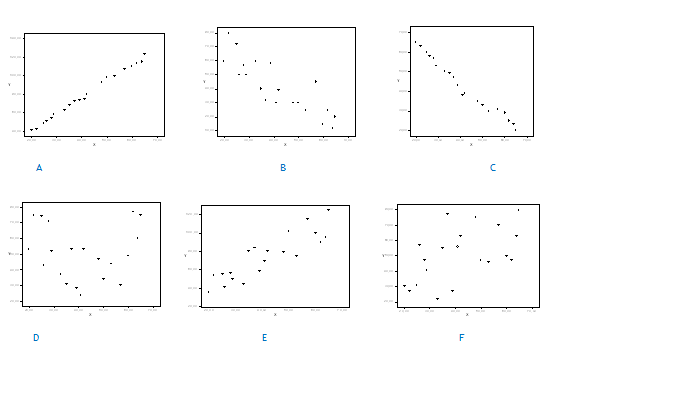
\includegraphics[width=1.10\textwidth]{correlaties.png}
  \captionof{figure}{Scatter plots of six data sets.}
  \label{fig:correlations}
  %\end{figure}
\end{exercise}

\begin{exercise}
  \label{ex:cats}
  Import the data set ``Cats.csv''.
  \begin{enumerate}
    \item Perform a linear regression analysis on the variables body weight (\texttt{Bwt}, dependent variable) and heart weight (\texttt{Hwt}, independent variabele).
    \item Draw a scatter plot of both variables.
    \item Calculate and draw the regression line.
    \item Calculate the correlation coefficient and the coefficient of determination.
    \item Interpret the results from the previous steps.
  \end{enumerate}
\end{exercise}

\begin{exercise}
  \label{ex:cats-sex}
  Use the same data set as in Exercise~\ref{ex:cats}.
  \begin{enumerate}
    \item Perform a linear regression analysis on the variables body weight (\texttt{Bwt}) and heart weight (\texttt{Hwt}), but this time \emph{subdivided by gender} (\texttt{Sex}).
    \item Draw a scatter plot of both variables for each gender.
    \item Calculate and draw the regression line.
    \item Calculate the correlation coefficient and the coefficient of determination.
    \item Interpret the results from the previous steps.
  \end{enumerate}
\end{exercise}

\begin{exercise}
  \label{ex:pizza}
  Import the data set ``Pizza.csv'' in R.
  \begin{enumerate}
    \item Perform a complete linear regression analysis on the variables  Rating and CostPerSlice. Draw the right conclusions and verify them using a plot.
    \item Investigate a possible relationship between Rating and Neighborhood. Which method can be used for this? Can you use the Rating data in the same form?
    \item Interpret the results.
    \item Represent the cross table using a bar chart. Also add a legend.
  \end{enumerate}
\end{exercise}


%%%%%%%%%%%%%%%%%%%%%%%%%%%%%%%%%%%%%%%%%%%%%%%%%%%%%%



\section{Solutions to selected exercises}
\label{ssec:bivariate-analysis-solutions}

\paragraph{Exercise~\ref{ex:music-wine-analysis}}

$\chi^2 \approx 18.2792$, Cramér's $V \approx 0.1939$

\paragraph{Exercise~\ref{ex:chisq-survey}}

\begin{enumerate}
  \item \texttt{Exer}/\texttt{Smoke}: $\chi^2 = 5.4885$, $g = 12.59159$, $p = 0.4828422$
  \item \texttt{W.Hnd}/\texttt{Fold}: $\chi^2 = 1.581399$, $g = 5.9915$, $p = 0.454$
  \item \texttt{Sex}/\texttt{Smoke}: $\chi^2 = 3.554$, $g = 7.8147$, $p = 0.314$
  \item \texttt{Sex}/\texttt{W.Hnd}: $\chi^2 = 0.236$, $g = 3.8415$, $p = 0.627$
\end{enumerate}

\paragraph{Exercise~\ref{ex:chisq-aids2}} $\chi^2 = 1083.372914$, $g = 14.067140$, $p \approx 1.157 \times 10^{-229}$

\paragraph{Exercise~\ref{ex:chisq-digimeter}} $\chi^2 \approx 6.6997$ ($df = 6$), $g \approx 12.5916$, $p \approx 0.3495$


\paragraph{Exercise~\ref{ex:casus-akin2016-toets}}

Table~\ref{tab:akin2016-results-t-test} provides an overview of the best and second best persistence type for each data size (based on the sample mean). The conclusion of~\textcite{Akin2016}, which states that \emph{Realm} is the most efficient persistence type, still holds, but for the small data sets the difference is not significant.

Note that we have not explicitly selected a specific significance level in advance. However, for $\alpha = 0.1$, $0.05$ or even $0.01$, the same conclusion can be drawn.

\begin{table}
  \begin{center}
    \begin{tabular}{llll}
      \toprule
      \textbf{Data Size} & \textbf{Best} & \textbf{2nd Best} & \textbf{$p$-value} \\ \midrule
      Small            & Realm          & SharedPreferences & 0.1699     \\
      Medium           & Realm          & GreenDAO          & 0.0002506  \\
      Large            & Realm          & SQLite            & 0.0017     \\ \bottomrule
    \end{tabular}
  \end{center}
  \caption{Results of the $t$-test for the best and second best persistence type, based on the sample mean~\autocite{Akin2016}.}
  \label{tab:akin2016-results-t-test}
\end{table}

\paragraph{Exercise~\ref{ex:test-examen}}

\begin{itemize}
  \item $\beta_{0} \approx 0.6333$, $\beta_{1} \approx 0.9667$
  \item $Cov \approx 6.444$, $R \approx 0.9352$, $R^2 \approx 0.8747$
\end{itemize}

\paragraph{Exercise \ref{ex:cats} and \ref{ex:cats-sex}}

\begin{center}
  \begin{tabular}{lrrrrr}
  	\toprule
    \textbf{Selection} & \textbf{$\beta_{0}$} & \textbf{$\beta_{1}$} & \textbf{$Cov$} & \textbf{$R$} & \textbf{$R^2$} \\
    \midrule
  	Full dataset & -0.3511 & 4.0318 & 0.9496 & 0.8041 & 0.6466 \\
  	Female       &  2.9813 & 2.6364 & 0.1979 & 0.5320 & 0.2831 \\
  	Male         & -1.1768 & 4.3098 & 0.9419 & 0.7930 & 0.6289 \\
    \bottomrule
  \end{tabular}
\end{center}

